
\section{Size Limits (lower bounds) for Effective Transfer Learning}
\label{sec:sizelimit}

Like prior works\cite{nam2013transfer,
  ma2012transfer, rahman2012recalling, ryu2014value,
  zhang2014towards}, the basic HDP method we
proposed above uses {\em all} the instances in potential source and target data to
perform KS-test to select the best matched metrics and then build
defect prediction learners.
Collecting {\em all} that data from source and target project need much more work and also
for the target project, it requires waiting for it to finish before
transferring its learned lessons. This begs the question ``how early can we transfer?''.
That is, how {\em few} data from source and target projects do we need before transfer can be effective?

\begin{figure}[t]
	\centering
% 	\vspace{0.5mm}
	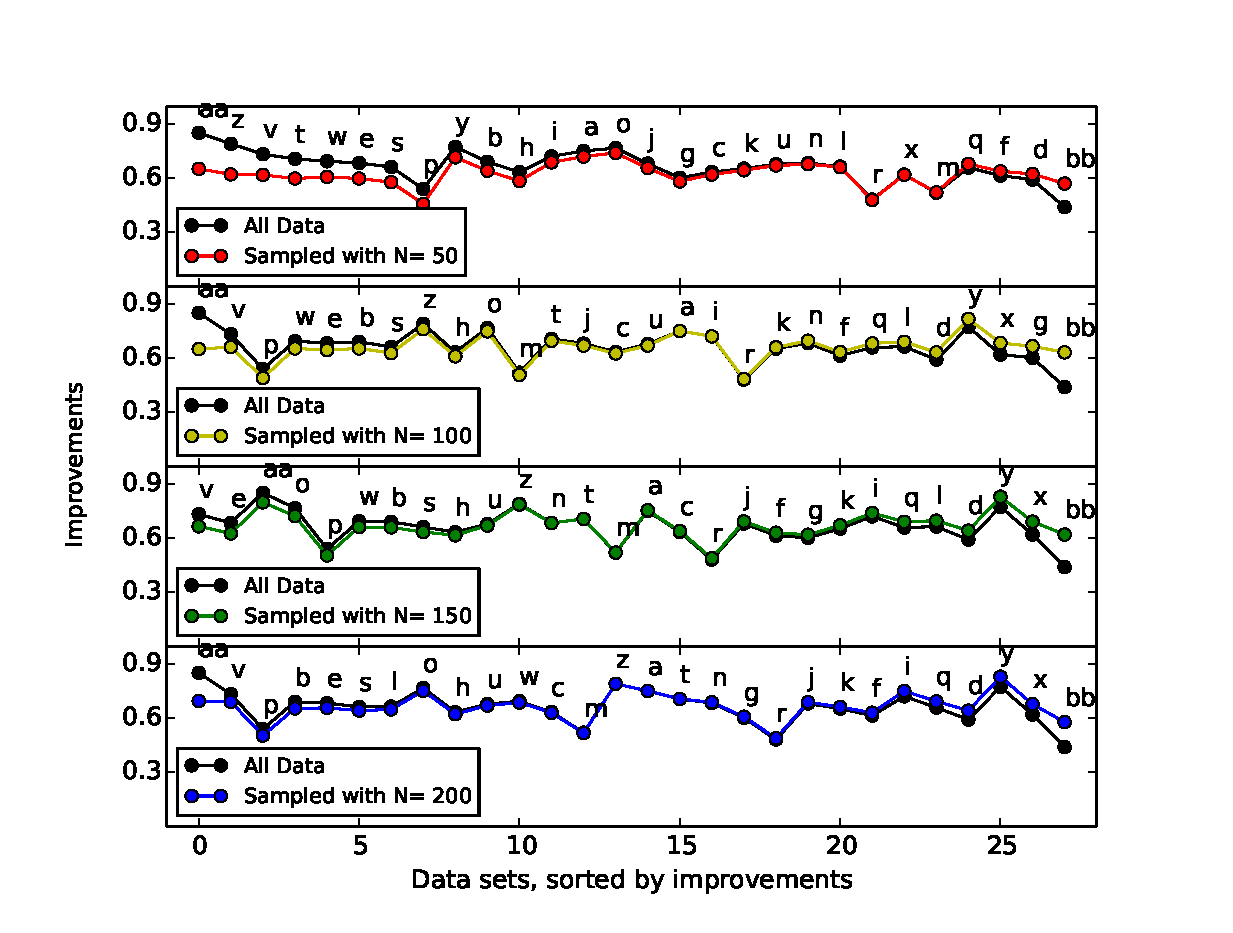
\includegraphics[width=\linewidth]{Figures/raleigh/sample_random.eps}
	\caption{Improvements of using sampled data over all data with sampled size N = \{50, 100, 150, 200\}. We label the data in table \ref{tab:datasets} from a to z, and the last two data sets ar5 and ar6 as A and B.}
	\label{fig:small_data}
\end{figure}


\subsection{200 Random Samples are Enough}

Recall from the above,
HDP uses  data sets  in a two step process.
To test the impact of having access to {\em less} data,
we  add a third initial sampling process before doing metric matching:
instead of using all the instances from
candidate source and target data sets, those data sets will
be randomly sampled to generate smaller data sets of
size $N \in \{50, 100, 150, 200\}$. If
the number of instances in the original data set is
smaller than $N$, all those instances will be
included. With those sampled data, we do metric matching to build learner
and finally predict labels of the original all data in target project.

The results for this HDP-with-limited-data experiment is shown in \fig{small_data}
(we display median AUC results from 20 repeats, using  Logistic regression
as the default learner). 
% Since {\it Apahce commons math} library takes quite long time to conduct KS-test as mentioned, we replace it with Scipy, a python package, to speed up our experiment. \footnote{As shown in the table, the difference between those two KS-test results is acceptable}.
In that figure:
\bi
\item
  The {\em black} line show the results using {\em all} data;
\item
  The {\em colourful} lines show results of transferring from {\em some} small $N$ number of samples(instead of {\em all})
  in the source and target data sets during metric matching and learner building;
\item
  The letters show the unique ID of each data set.
\ei
The data sets are ordered left to right by the difference to the black line (where we transfer using {\em
  all} the source data):
\bi
\item
  On the left, the black line is
  {\em above} the red line; i.e. for those data sets, we do {\em better} using
  {\em all} data than using {\em some}.
  \item
On the right, the black line is {\em below} the red
line; i.e. for those data sets, we do {\em worse}
using {\em all} data than using {\em some}.  \ei
Note that the gap between the red and black line
shrinks as we use more data and after $N=100$, the
net gap space is almost zero.  When $N=200$, $27/28$
tests are within 0.05 difference in terms of AUC and
$17/28$ tests show smaller data sets have equivalent
or even better performance. Here, we recommend that
sample size $N=200$ could be good enough for this
HDP framework to get a good predictor.



\begin{figure}[t]
	\centering
% 	\vspace{0.5mm}
	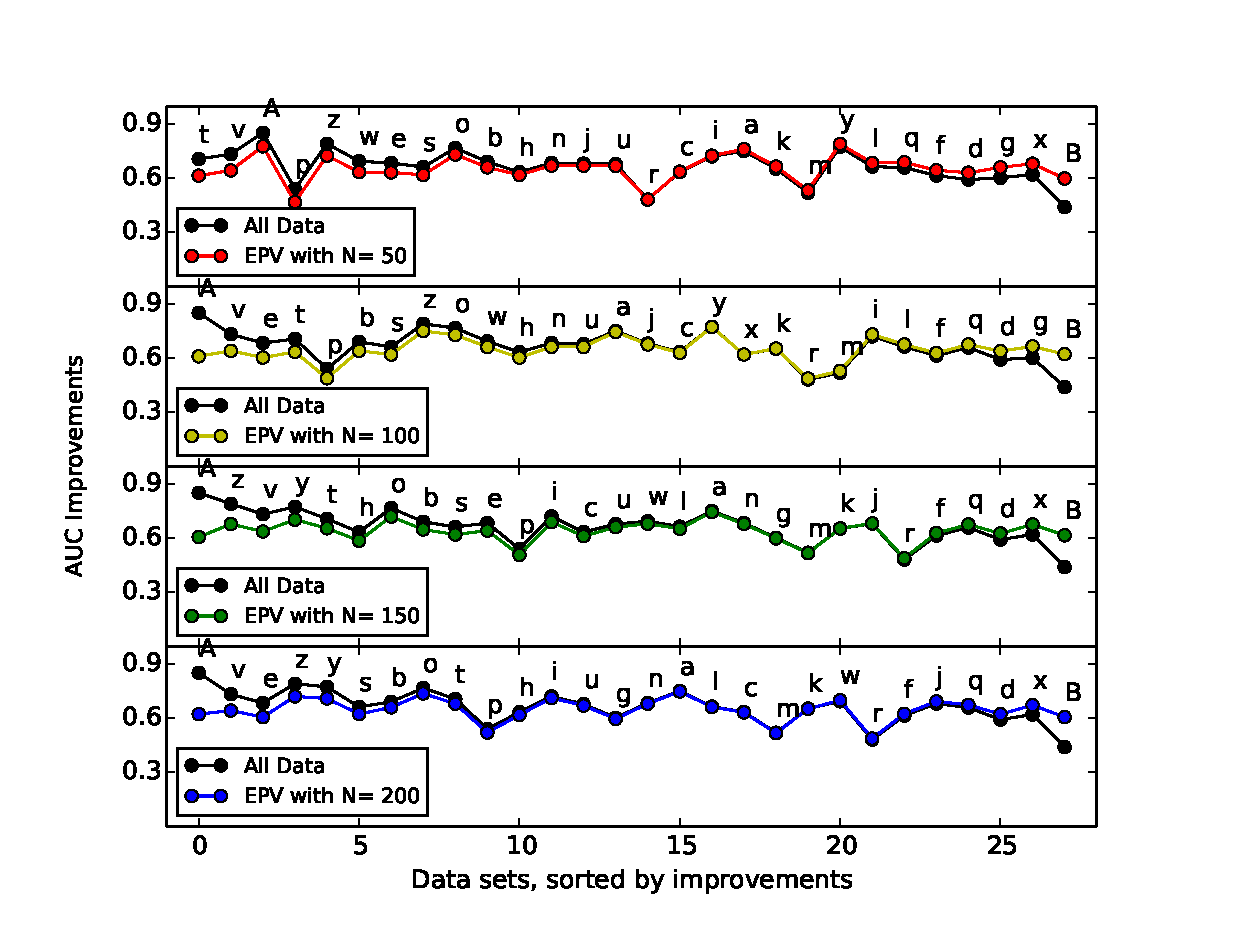
\includegraphics[width=\linewidth]{Figures/raleigh/sample_epv.eps}
	\caption{Improvements of using sampled data N = \{50, 100, 150, 200\} with EPV constraints. We label the data in table \ref{tab:datasets} from a to z, and the last two data sets ar5 and ar6 as A and B.}
	\label{fig:small_epv}
\end{figure}


\subsection{20 Defective Examples  are Enough}


The results of the last section are very encouraging-- a small number of source
and target examples are enough for effective transfer learning. Naturally,
we were suspicious of this result (since it was ``almost too good to be true'').
Accordingly, we explored the literature and found:
\bi
\item Evidence that this ``a few examples are enough'' has been seen in other domains;
\item Methods to reduce the cost of reducing this data set, even further.
  \ei
Working in the domain cardiology,
  Peduzzi et al.~\cite{peduzzi1996simulation}
  report 10 ``events'' per variable (EPV) are enough to maximize the predictive performance
  of  Logistic Regression (the learner used in this study). Translated into our terminology,
  that study would predict that  10 defective data per independent variable should
  suffice for effective learning. Of course, learners require defective and {\em non-defective}
  examples so to $M$ defective examples, we add $(N-M)$ non-defective examples more.

  To apply the method of Peduzzi et al., we first instrumented HDP to determine how many
  independent variables were picked during {\em metric  selection}. In practice, that number
  was very small: usually just 2. Hence, applying  Peduzzi et al.'s rule, we picked $2*10=20$
  randomly selected defective data, then randomly added $(N-M)$ non-defective data for
  $N\in \{50,100,150,250\}$ for the source data. For the target data set, since we don't
  know the labels of data, we simply sampled $N$ for target data in metric matching.

  (Aside: note that this is different to the above experiment since, before, the more $N$ examples
  we selected, the more {\em defective} modules we would use. Now, in this experiment, we will also
  use a fixed $M=20$ number of defects.).

  The results are shown in \fig{small_epv}. Like before:
  \bi
  \item These are median AUC results from 20 repeats;
\item
  The {\em black/colourful} lines show the results using {\em all/some} of  data from
  the source and target data sets during metric matching and learner building, respectively
  (but now, the {\em some} never contains more than $M=20$ defective modules);
\item
  The data sets are ordered left to right according
  the performance difference between using
   {\em all} or {\em some} of the data;
   \item
     On the left/right ,  we do {\em better/worse} using
  {\em all} data than using {\em some}.
  \ei
  We observe that between $N=50$ and $N=200$, the performance delta
  does not change by very much. Also, if we compare $N=200$ between \fig{small_data}
  and \fig{small_epv}, there seems no large disadvantage of using just
  $M=20$ defective modules.

  Note that such a very small sample would be very quick to collect: after writing (say) a few
  hundred classes, inspect enough to find 20 defective ones---at which point that data is a candidate
  for transfer learning.
